\vspace{10pt}

{\centering\subsection*{白水:从路过书架开始的阅读}}

\addcontentsline{toc}{subsection}{白水:从路过书架开始的阅读}

\renewcommand{\leftmark}{白水:从路过书架开始的阅读}

\begin{figure}[htbp]

\centering

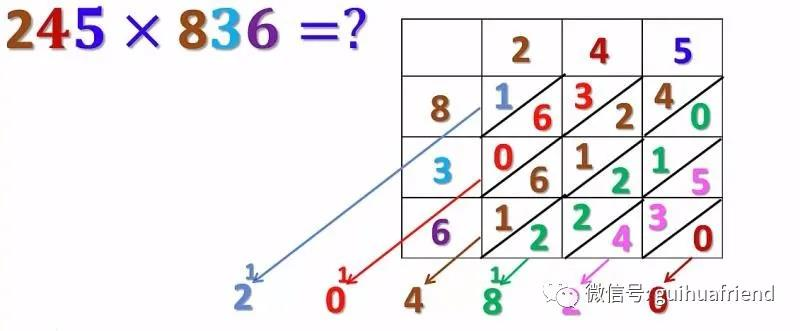
\includegraphics[width = .5\textwidth]{./ch/v5.jpg}

\end{figure}

与你共同成长。



你好,这里是桂花图书馆阅读分享,我是馆长莫静琴。



通过图书馆读者家长群的分享,我们观察到,有的同学阅读集中在优秀作文集,有的同学试图多阅读经典文学作品。小学生的阅读,阅读的目标和如何选书似乎是一个问题。我们想在这里进行探讨。



首先,从功利或者务实的角度,阅读长期来看是有利于提高学习成绩的,但是这里面的原因可能要梳理。



中国的小学生课业已经够重了,图书馆的目标绝不是又增加一门课,增加新的负担。变成负担的方式可以是,家长期待孩子把书里面的内容记住,从而希望马上能应用到考试里面,提高考试成绩。记住好词好句,或许的确能提高写作中的词汇的水平,但是可能无助于提高写作的逻辑能力。



写作能力,更加关键在于采集大量的生活中的素材,以及大量的写作练习和反馈。我自身的例子,小学摘抄的好词好句现在全无印象。但是,六年级时,太热突然暴雨,天气变凉爽,随意写的打油诗;因为班长受伤,写下自己当时的感受的几句日记,却至今有模糊的印象。



阅读能力是一种学习能力,能提高学科学习效果,是因为大量的阅读,锻炼了理解文本和概念的能力。理解文本和概念的能力,是任何一门学科的基础能力。



阅读如果不需要记忆,那需要做啥呢?图书馆期待的一种阅读,是基于好奇心的阅读,是自主的阅读。



走进图书馆,打开书,就应该像是在小溪翻开石块找螃蟹一样的过程,一样的体会。学习中,生活中,有啥不懂的,有啥好奇的,教科书上没有的,老师没讲的,完全可以去自己找更多的书籍资料阅读。我小学时候着迷数学,就迫不及待的想了解更多,当时有机会去新华书店能呆上半天。通过家里愿意买的数学小册子,了解到的一种基于格子的乘法方式,而且也了解到十进制之外的二进制。这些课本之外自主探索的知识,越发加强了我的数学上的兴趣。所以阅读,是需要由好奇心驱动的。



最后,阅读是在阅读啥呢?图书馆为何要用这么高的运营成本来请馆长专职维持开馆呢?



阅读是读文字么?是的,但是这可能不是阅读的全部。绝大部分的书籍是不需要精读的。阅读首先是读书架,读书侧面的标题,读封面,读目录。只有极少数的那些和好奇心和困惑相关的书籍,才需要去精读。阅读不是看文字的任务,而是一种像翻字典一样找到答案,探索和寻找自己想要的信息的游戏。



图书馆的布局,和班级图书角的布局差别在哪里?图书馆的布局,又和家里的书架的布局差别在哪里?是书籍数量的差别么?是的。但是一两个数量级的差别,导致的是书籍丰富性的本质差别。阅读,从走进图书馆开始,从路过书架扫读书籍开始,从借出一本开始,从翻开一本书的目录开始。所以,走进图书馆吧,开始珍贵的阅读。



这是我们这周的分享。谢谢大家。

\vspace{10pt}



文稿:白水

朗读:莫静琴

发布:2021年5月9日








\vspace{10pt}

\hline

